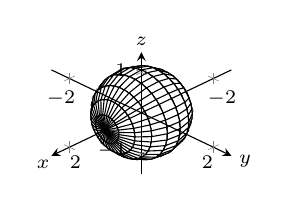
\begin{tikzpicture}[>=stealth]
\begin{axis}%
[width=175pt,tick label style={font=\scriptsize},axis on top,
			axis lines=center,
			view={135}{45},
			name=myplot,
			%xtick={2},
			%ytick={-4,2,4},
			%ztick={-4,2,4},
			ymin=-2.5,ymax=2.5,
			xmin=-2.5,xmax=2.5,
			zmin=-1.5, zmax=1.5,
			every axis x label/.style={at={(axis cs:\pgfkeysvalueof{/pgfplots/xmax},0,0)},xshift=-3pt,yshift=-3pt},
				xlabel={\scriptsize $x$},
			every axis y label/.style={at={(axis cs:0,\pgfkeysvalueof{/pgfplots/ymax},0)},xshift=5pt,yshift=-2pt},
				ylabel={\scriptsize $y$},
				every axis z label/.style={at={(axis cs:0,0,\pgfkeysvalueof{/pgfplots/zmax})},xshift=0pt,yshift=4pt},
				zlabel={\scriptsize $z$}
			]



%\addplot3[domain=-2:2,,y domain=-2:2,surf,faceted color={\coloronefill},samples=10,colormap={mp2}{\colormapplaneone}] {(x^3-2*x)};

%\addplot3[domain=0:360,,y domain=0:360,surf,faceted color={\coloronefill},samples=30,colormap={mp2}{\colormapplaneone},z buffer=sort] ({cos(x)},{sin(x)*cos(y)},{sin(x)*sin(y)});

\addplot3[domain=0:360,smooth,y domain=0:360,surf,fill=white,faceted color=black,samples=20,,z buffer=sort] ({cos(x)},{sin(x)*cos(y)},{sin(x)*sin(y)});



\end{axis}

\end{tikzpicture}










